% ===========================================
% Data Processing
% Written by: Braidan Duffy
%
% Date: 06/22/2022
% Last Revision: 06/22/2022
% ============================================

\setchapterstyle{kao}
\chapter{Data Processing}
\setchapterpreamble[u]{\margintoc}
\labch{data_processing}
% \addcontentsline{toc}{chapter}{Data Processing} % Add the preface to the table of contents as a chapter

Data collected from sensors can sometimes be useful on their own, but often times, it is necessary to process it to gain a better understanding of what is occurring.
To that end, this chapter will be about how to process raw data into something more usable and some techniques that you can employ for your projects in the future.

    \section{Digital Filtering} \labsec{digital_filtering}
    One of the most fundamental data processing techniques is that of the digital filter.
    The idea behind these filters is to take in data samples and apply mathematical formulations on them to dampen undesirable signals within.
        
        \subsection{Background} This section assumes that you do not have a lot of background knowledge on basic statistics and terminology.
        It is important to understand here that mean and expected value are not the same thing.
        In many college lab courses, measurements are taken multiple times and averaged together to find the mean value (often denoted as $\mu$).
        This is assumed to be the absolute correct value with zero uncertainty.
        However, this is never the case in the real world as all measurements have uncertainty in some fashion.
        When the average measurement value is taken \textit{with} uncertainties factored in, this becomes the expected value ($E$) and used to guess what the real (correct) value of the measured variable is.

        So, how can quantify the uncertainties within the expected value? First, we need to know what the measurement variance is.
        This value is a description of how far the measured data is from the mean and is defined in Equation \ref{eq:variance}. \sidenote{For large datasets, variance is normalized by $\frac{1}{N-1}$}

        \marginnote{The standard deviation of the dataset $\sigma$ decribes the probabalistic distance a measurement can have from the mean and is defined by:
        \begin{equation*}
            \sigma = \sqrt{\sigma^2}
        \end{equation*}
        }
        
        \begin{gather} \labeq{variance}
            \sigma^2 = \frac{1}{N} \sum_{n=1}^{N} (x_n - \mu)^2 \\ 
            \begin{aligned}
                \text{where } &\sigma^2 \text{ is the variance} \\
                &N \text{ is the total number of samples} \\
                &x_n \text{ is the n-th sample} \\
                &\mu \text{ is the running average}
            \end{aligned} \notag
        \end{gather}

        \begin{kaobox}[frametitle=Aside: Normal Distribution]
            Normal distribution of data is the archetypical bell curve.
            It is also referred to Gaussian distribution and is defined by:
            \begin{equation*}
                f(x, \mu, \sigma^2) = \frac{1}{2\pi\sigma^2} \exp{\frac{-(x-\mu)^2}{2\sigma^2}}
            \end{equation*}
            This function creates a Gaussian curve which is the Probability Density Function (PDF) for a normal distribution.
            Normally, measurements errors are Gaussian-distributed and the Kalman filter assumes this is always the case.
            Different error distributions will drastically increase the uncertainties within the filter and may negate it entirely.
        \end{kaobox}
        
        \begin{marginfigure}[-2in]
            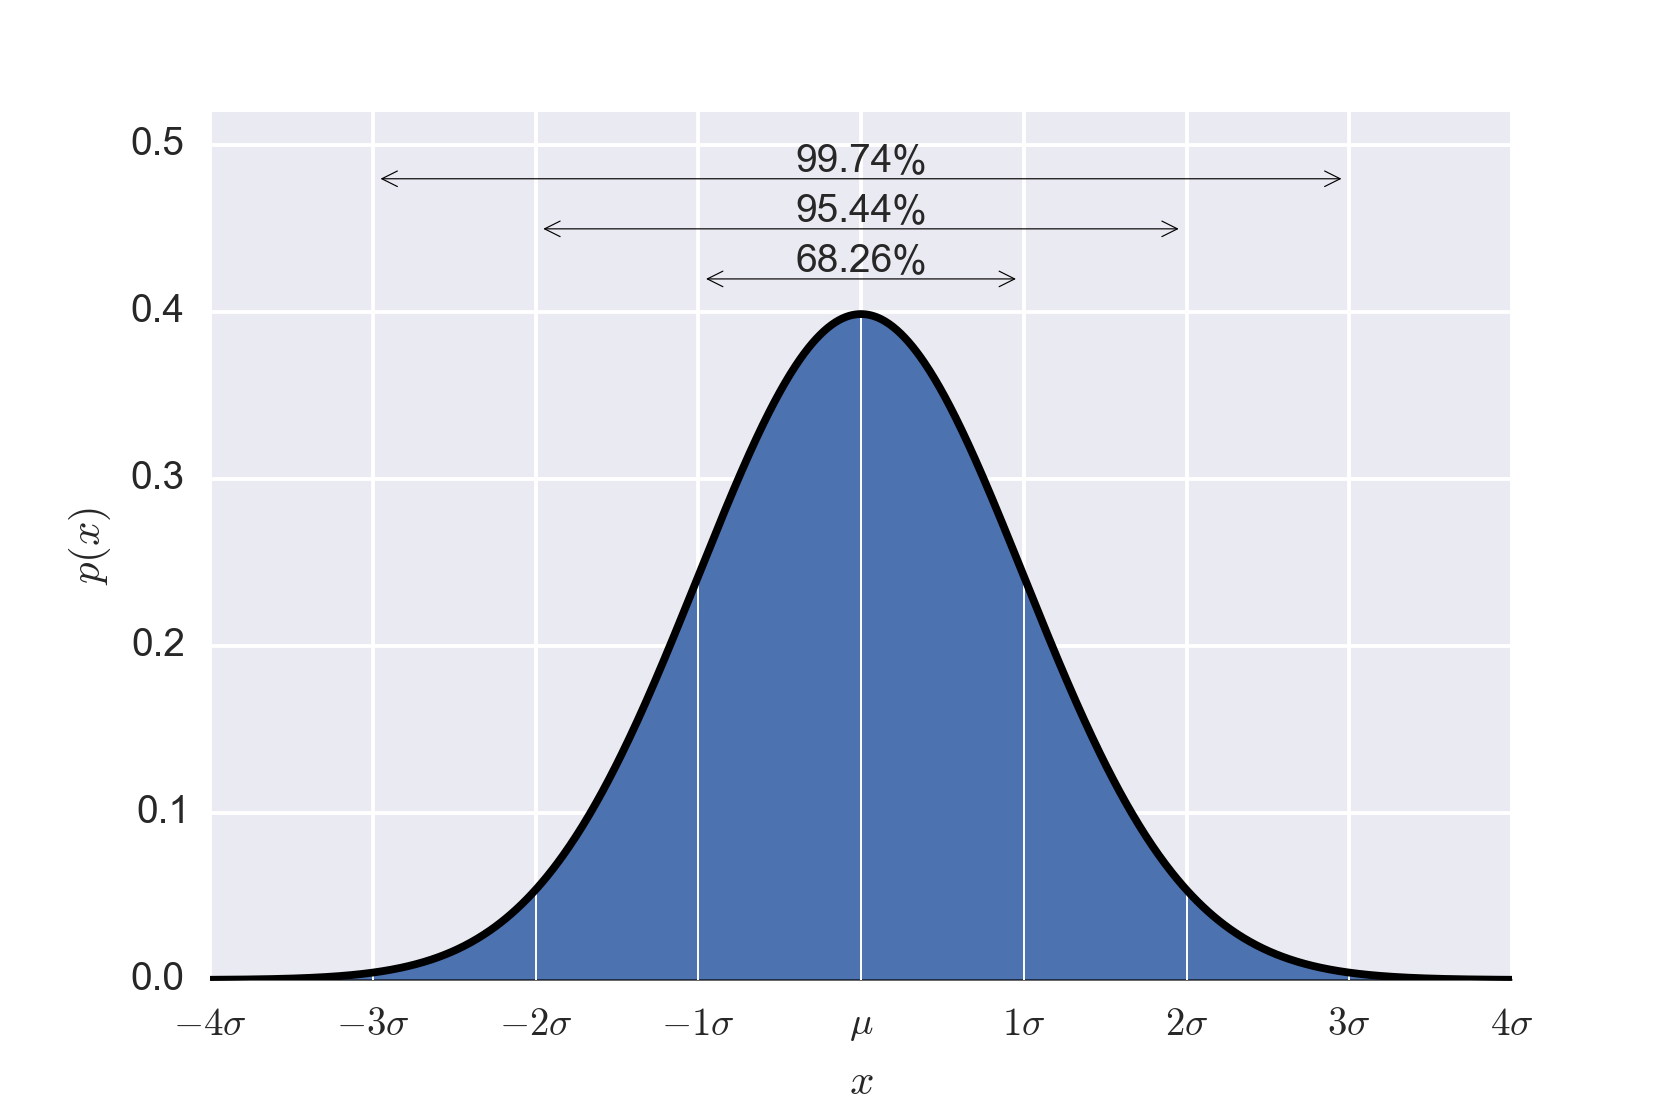
\includegraphics[]{data_processing/gaussian_distribution.png}
            \caption[Aside: Gaussian Distribution]{A graph of a Gaussian distribution with the 1st standard deviations shown.
            Retrieved from \href{https://accadandkoka.com/blog/how-normal-is-the-normal-distribution/}{The Akkad and Koda Report}}
            \labfig{aside_gaussian_dist}
        \end{marginfigure}

        Estimates are the algorithm's guessed value at the unknown system state.
        Here, accuracy quantifies how close the estimate is to the true value whereas precision quantifies the variability of the estimates with respect to uncertainty.
        High precision estimates have a low variance (uncertainty) in measurements.
        Low accuracy estimates display a bias that are systemic errors in measurement.
        Variance is determined by random measurement error and can be reduced by averaging or smoothing the measurements.

        \begin{figure*}[h!]
            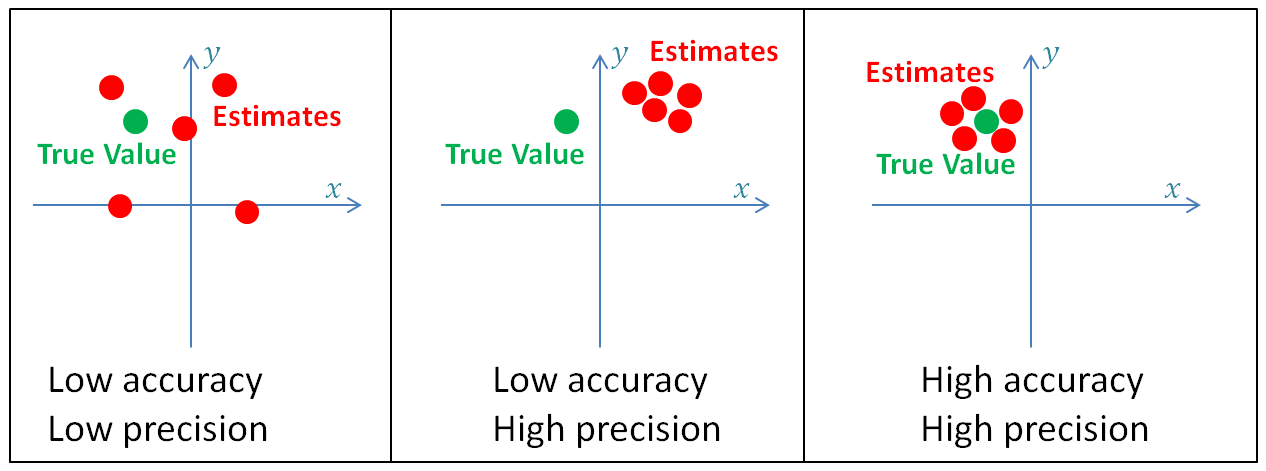
\includegraphics[]{data_processing/AccuracyAndPrecision.png}
            \caption[Accuracy and Precision]{Different plots demonstrating the difference between accuracy and precision.
            Retrieved from \href{https://www.kalmanfilter.net/img/BB1/AccuracyAndPrecision.png}{KalmanFilter.net}}
            \labfig{accuracy_precision}
        \end{figure*}

        \subsection{The $\alpha$ Filter} 
        At any sample, $N$, a value $\hat{x}_{N,N}$ can be estimated using:
        
        \begin{gather*} \labeq{sample_estimate}
            \hat{x}_{n,n} = \frac{1}{N} \sum_{n=1}^{N} (z_n) \\
            \begin{aligned}
                \text{where } &\hat{x}_{n,n} \text{is the estimate of the true value at sample $n$} \\
                &N \text{ is the total number of samples taken} \\
                &n \text{ is the current sample number} \\
                &z \text{ is the current measurement} \\
            \end{aligned} \notag
        \end{gather*}

        Since the estimate accuracy will improve with the number of measurements, we need to remember all the historical measurements.
        However, storing, accessing, and operating on discrete measurements exponentially increases in difficulty and computational power as more measurements are taken.
        Therefore, we can store the previous measurements in a state variable and add a small adjustment that is proportional to the newest measurement.
        This preserves the accuracy of storing many discrete data points and the computing and storage resources required to operate on data added to the set.

        This algorithm is called the \textit{State Update Equation} and is one of the five Kalman equations. 
        It is defined by:

        \begin{gather} \labeq{state_update_eq}
            \hat{x}_{n,n} = \hat{x}_{n,n-1} + \alpha_n(z_n - \hat{x}_{n,n-1}) \\
            \begin{aligned}
                \text{where } &\hat{x}_{n,n} \text{is the estimate of the true value at sample $n$} \\
                &\hat{x}_{n,n-1} \text{ is the estimate of the previous true value} \\
                &n \text{ is the current sample number} \\
                &\alpha_n \text{ is a correction gain} \\
                &z \text{ is the current measurement} \\
            \end{aligned} \notag
        \end{gather}

        \marginnote[-1.5in]{The correction gain, $\alpha_n$ is unique to every example and can change with every sample.
        It is also called the Kalman gain, denoted by $K_n$}

        \marginnote[-0.75in]{The term $(z_n - \hat{x}_{n,n-1})$ is the measurement residual or "innovation"; this contains the new information.}

        This algorithm uses zero-indexing, so the initial or starting guess will be $n=0$.
        This value can be determined by reasoning or physical constraints of the system.
        The filter will always require an initial guess to kickstart the algorithm.
        A flow chart describing the algorithm's process is below.

        \todo{INSERT ALPHA FILTER FLOW CHART HERE!}
        
        \pagelayout{wide} % No margins

        \begin{example} \label{ex:alpha_filter}
        Let's say that we are programming a scale to estimate the weight of an ROV placed atop it.
        For the sake of example, we know that the ROV weighs exactly 10 kilograms and we want to quantify the uncertainty of our scale.
        \paragraph{Iteration 0}
        \begin{equation*}
            \begin{aligned} 
                0:& \text{ We can guess that the initial weight of the ROV is 10-kg: } \hat{x}_{0,0} = 10 \text{ kg} \\
                3:& \text{ Since the weight should not change, our prediction for the next measurement is: } \hat{x}_{1,0} = \hat{x}_{0,0} = 10 \text{ kg} \\
            \end{aligned}
        \end{equation*}
        
        \paragraph{Iteration 1}
        \begin{equation*}
            \begin{aligned} 
                1:& \text{ We make a measurement on the scale: } z_1 = 10.3 \text{ kg} \\
                2\text{a}:& \text{ We calculate the correction gain: } \alpha_1 = \frac{1}{N} = \frac{1}{1} = 1 \\
                2\text{b}:& \text{ We can then estimate the current state: } \hat{x}_{1,1} = \hat{x}_{1,0} + \alpha_1(z_1 - \hat{x}_{1,0}) = 10 + 1(10.3 - 10) = 10.3 \text{ kg} \\
                3:& \text{ Since the weight should not change: } \hat{x}_{2,1} = \hat{x}_{1,1} = 10.3 \text{ kg} \\
            \end{aligned}
        \end{equation*}

        \paragraph{Iteration 2}
        \begin{equation*}
            \begin{aligned} 
                1:& \text{ We make a measurement on the scale: } z_2 = 9.9 \text{ kg} \\
                2\text{a}:& \text{ We calculate the correction gain: } \alpha_2 = \frac{1}{N} = \frac{1}{2} = 0.5 \\
                2\text{b}:& \text{ We can then estimate the current state: } \hat{x}_{2,2} = \hat{x}_{2,1} + \alpha_2(z_2 - \hat{x}_{2,1}) = 10.3 + 0.5(9.9 - 10.3) = 10.1 \text{ kg} \\
                3:& \text{ Since the weight should not change: } \hat{x}_{3,2} = \hat{x}_{2,2} = 10.1 \text{ kg} \\
            \end{aligned}
        \end{equation*}

        The calculations and results for this example are summarized in the table and figure below:

        \begin{center}
            \begin{tabular}{c | c | c | c | c}
            \toprule
            & \multicolumn{3}{|c|}{Current Estimates} & Predictions \\
            \midrule
            n & $z_n$ & $\alpha_n$ & $\hat{x}_{n,n}$ & $\hat{x}_{n+1,n}$ \\
            \midrule

            0  & ---- &      ----      & 10.0 & 10.0 \\[4pt]
            1  & 10.3 &       1        & 10.3 & 10.3 \\[4pt]
            2  &  9.9 & $\frac{1}{2 }$ & 10.1 & 10.1 \\[4pt]
            3  &  9.8 & $\frac{1}{3 }$ & 10.0 & 10.0 \\[4pt]
            4  & 10.3 & $\frac{1}{4 }$ & 10.1 & 10.1 \\[4pt]
            5  & 10.4 & $\frac{1}{5 }$ & 10.1 & 10.1 \\[4pt]
            6  & 10.1 & $\frac{1}{6 }$ & 10.1 & 10.1 \\[4pt]
            7  & 10.3 & $\frac{1}{7 }$ & 10.2 & 10.2 \\[4pt]
            8  & 10.0 & $\frac{1}{8 }$ & 10.1 & 10.1 \\[4pt]
            9  &  9.8 & $\frac{1}{9 }$ & 10.1 & 10.1 \\[4pt]
            10 &  9.5 & $\frac{1}{10}$ & 10.0 & ---- \\[4pt]

            \bottomrule
            \end{tabular}
        \end{center}

        \begin{center}
            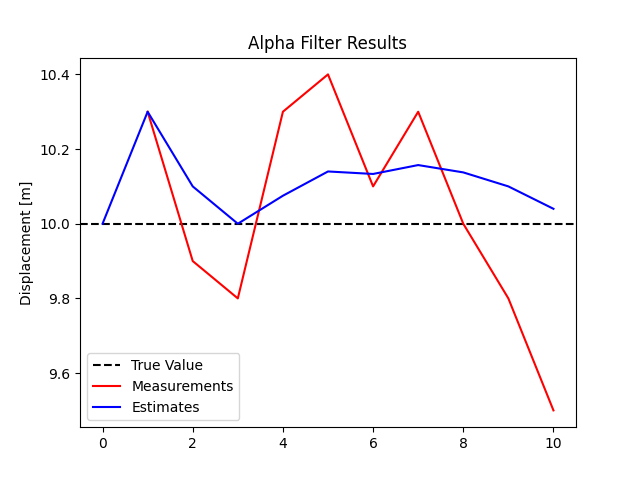
\includegraphics[height=3.5in]{examples/alpha_filter_results.png}
        \end{center}

        The $\alpha$-filter considerably smoothed out the noisy measurement data and will eventually converge on an estimate close to the true value (within 10\%).

        \end{example}

        \pagelayout{margin} % Replace margins

        \subsection{The $\alpha$ and $\beta$ Filter}
        As demonstrated in Example \ref{ex:alpha_filter}, the $\alpha$ filter makes a major assumption that the state does not change between samples.
        In reality, this is rarely the case as we typically want to measure a body's movement, or track a variable over time, or measure something that has dependency on another variable.
        
        For example, if we wished to track a boat moving in a one-dimensional world at a constant velocity (no acceleration), we need to modify our model a bit.
        For nomenclature, $x_n$ will represent the displacement of the vessel from a known starting point.
        Since the vessel is moving with a constant velocity, we can model its time rate of change of position as:
        
        \begin{equation*}
            \dot{x} = v = \frac{dx}{dt}
        \end{equation*}

        If we sample the vessel's displacement at intervals of $\Delta t$ time, then we can define a dynamic model of the vessels movement as:

        \begin{subequations}
            \labeq{see_dynamic_model}
            \begin{align}
                x_{n+1} &= x_n + \Delta t \dot{x}_n \labeq{see_disp}\\
                \dot{x}_{n+1} &= \dot{x}_n \labeq{see_velocity}
            \end{align}
        \end{subequations}

        This is called the \textit{State Extrapolation Equation} \sidenote{or the \textit{State Transistion Equation} or the \textit{State Prediction Equation}} and is another one of the five Kalman equations.
        If we assume the sample interval is $\Delta t = 5 \text{ seconds}$ at sample $n-1$ and the displacement and velocity of the vessel is estimated as 300-m and 10-m/s, respectively, then using Equations \ref{eq:see_disp} and \ref{eq:see_velocity}, we can predict where the vessel will be and its velocity at sample $n$.
        
        \begin{equation*}
            \begin{gathered}
                \hat{x}_{n,n-1} = \hat{x}_{n-1,n-1} + \Delta t \hat{\dot{x}}_{n-1,n-1} = 300 + 5(10) = 350 \text{ m} \\
                \hat{\dot{x}}_{n,n-1} = \hat{x}_{n-1,n-1} = 10 \text{ m/s}
            \end{gathered}
        \end{equation*}

        However, at sample $n$, the vessel records a displacement of 320-m, not the expected 350-m; there are two possible reasons:

        \begin{enumerate}
            \item the vessel displacement measurements are not precise or accurate
            \item the vessel velocity changed unexpectedly \sidenote{The new velocity would have to be:
                                                                        \begin{equation*}
                                                                            \frac{320-300}{5} = 4 \text{ m/s}
                                                                        \end{equation*}}
        \end{enumerate}

        We know from the previous section that we can account for the measurement error using an $\alpha$ filter, so lets re-write Equation \ref{eq:see_velocity} to account for error in the velocity:

        \begin{equation}
            \labeq{see_velocity_b}
            \hat{\dot{x}}_{n,n} = \hat{\dot{x}}_{n,n-1} + \beta(\frac{z_n - \hat{x}_{n,n-1}}{\Delta t})
        \end{equation}

        \todo{INSERT FIGURE OF THE $\alpha$ - $\beta$ FILTER ALGORITHM}

        \pagelayout{wide} % Remove margins

        \begin{example} \label{ex:alpha_beta_filter}
        Consider a boat moving in one dimension. 
        We are going to assume the following:
        \begin{itemize}
            \item $\alpha = 0.2$ (Positional gain)
            \item $\beta = 0.1$ (Velocity gain)
            \item $\Delta t = 5$ seconds
        \end{itemize}

        \paragraph{Iteration 0}
        \begin{equation*}
            \begin{aligned} 
                0:& \text{ Initial conditions: } \hat{x}_{0,0} = 300 \text{ m, } \hat{\dot{x}}_{0,0} = 4 \text{ m/s} \\
                3:& \text{ Predict the next position: } \hat{x}_{1,0} = \hat{x}_{0,0} + \Delta t \hat{\dot{x}}_{0,0} = 300 + 5(4) = \textbf{320 m} \\
                 :& \text{ Predict the next velocity: } \hat{\dot{x}}_{1,0} = \hat{\dot{x}}_{0,0} = \textbf{4 m/s}
            \end{aligned}
        \end{equation*}
        
        \paragraph{Iteration 1}
        \begin{equation*}
            \begin{aligned} 
                1:& \text{ The vessel makes a positional measurement: } z_1 = \textbf{310 m} \\
                2:& \text{ We estimate the current position: } \hat{x}_{1,1} = \hat{x}_{1,0} + \alpha(z_1 - \hat{x}_{1,0}) = 320 + 0.2(310 - 320) = \textbf{318 m} \\
                 :& \text{ We estimate the current velocity: } \hat{\dot{x}}_{1,1} = \hat{\dot{x}}_{1,0} + \beta(\frac{z_1 - \hat{x}_{1,0}}{\Delta t}) = 4 + 0.1(\frac{310 - 320}{5}) = \textbf{3.8 m/s} \\
                3:& \text{ Predict the next position: } \hat{x}_{2,1} = \hat{x}_{1,1} + \Delta t \hat{\dot{x}}_{1,1} = 318 + 5(3.8) = \textbf{337 m} \\
                 :& \text{ Predict the next velocity: } \hat{\dot{x}}_{2,1} = \hat{\dot{x}}_{1,1} = \textbf{3.8 m/s}
            \end{aligned}
        \end{equation*}

        \paragraph{Iteration 2}
        \begin{equation*}
            \begin{aligned} 
                1:& \text{ The vessel makes a positional measurement: } z_2 = \textbf{317 m} \\
                2:& \text{ We estimate the current position: } \hat{x}_{2,2} = \hat{x}_{2,1} + \alpha(z_2 - \hat{x}_{2,1}) = 337 + 0.2(317 - 337) = \textbf{333 m} \\
                 :& \text{ We estimate the current velocity: } \hat{\dot{x}}_{2,2} = \hat{\dot{x}}_{2,1} + \beta(\frac{z_2 - \hat{x}_{2,1}}{\Delta t}) = 3.8 + 0.1(\frac{337 - 317}{5}) = \textbf{3.4 m/s} \\
                3:& \text{ Predict the next position: } \hat{x}_{3,2} = \hat{x}_{2,2} + \Delta t \hat{\dot{x}}_{2,2} = 333 + 5(3.4) = \textbf{350 m} \\
                 :& \text{ Predict the next velocity: } \hat{\dot{x}}_{3,2} = \hat{\dot{x}}_{2,2} = \textbf{3.4 m/s}
            \end{aligned}
        \end{equation*}

        The data for this example is summarized in the table and figure below:

        \begin{center}
            \begin{tabular}{c | c | c | c | c | c}
            \toprule
            & \multicolumn{3}{|c|}{Current Estimates} & \multicolumn{2}{c}{Predictions} \\
            \midrule
            n & $z_n$ & $\hat{x}_{n,n}$ & $ \hat{\dot{x}}_{n,n} $ & $ \hat{x}_{n+1,n}$ & $ \hat{\dot{x}}_{n+1,n} $ \\
            \midrule

            0  &  ---  & 300.0 & 4.00 & 320.0 & 4.00 \\
            1  & 322.0 & 320.4 & 4.04 & 340.6 & 4.04 \\
            2  & 341.0 & 340.7 & 4.05 & 360.9 & 4.05 \\
            3  & 358.0 & 360.3 & 3.99 & 380.3 & 3.99 \\
            4  & 374.0 & 379.0 & 3.86 & 398.3 & 3.86 \\
            5  & 399.0 & 398.5 & 3.88 & 417.9 & 3.88 \\
            6  & 420.0 & 418.3 & 3.92 & 437.9 & 3.92 \\
            7  & 436.0 & 437.5 & 3.88 & 456.9 & 3.88 \\
            8  & 458.0 & 457.1 & 3.90 & 476.7 & 3.90 \\
            9  & 483.0 & 477.9 & 4.03 & 476.7 & 4.03 \\
            10 & 501.0 & 498.7 & 4.09 & 498.1 & 4.03 \\

            \bottomrule
            \end{tabular}
        \end{center}

        \begin{center}
            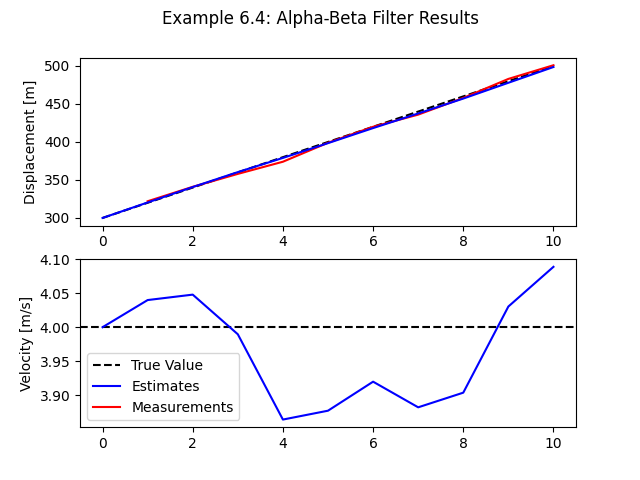
\includegraphics[height=3.5in]{examples/ex_6_4_alpha_beta_filter_results.png}
        \end{center}

        From the figure, we can see that the filter provides a good "smoothing" effort for the noisy measurement data.
        High values for $\alpha$ and $\beta$ will result in less "smoothing" in certain cases.
        The current state estimate may be very close to the measurement values with a higher error in predicted values

        The value of $\beta$ depends on the precision of the vessel's navigation system.
        If the positional precision is $\sigma = 0.1 \text{ m}$, then it is very likely the vessel speed changed.
        Therefore, $\beta$ would be very high to adjust the estimated velocity.
        Conversely, if the positional precision is $\sigma = 10 \text{ m}$, then it is likely the vessel's position measurements are wrong and $\beta$ can be smaller.

        $\alpha$ and $\beta$ depend on the measurement precision.
        Very precise measurements would prefer a high $\alpha$ and $\beta$ gains that will cause the filter to converge quickly and can adapt to velocity changes.
        Lower precision measurements would prefer lower $\alpha$ and $\beta$ gains that allow any uncertainties to be smoothed out; this will cause the filter to react slowly to velocity changes or external perturbations, though.
        
        \end{example}

        \pagelayout{margin} % Restore margins

        \paragraph{The Importance of Accurate Modelling} Lets expand upon Example \ref{ex:alpha_beta_filter}.
        Here, we will consider the same vessel under the same assumptions and initial conditions, but we will have a flawed dynamic model.
        The vessel will begin transiting at a constant velocity of 5-m/s for 15 seconds, then accelerate at a constant 2-m/s/s for 15 seconds.
        The kinematic plots are displayed below in Figure \ref{} and the numerical results can be found in Table \ref{}.

        \todo{INSERT KINEMATIC GRAPH FIGURE SHOWING VESSEL ACCELERATION, VELOCITY, AND DISPLACEMENT OVER TIME}

        \todo{INSERT TABLE OF NUMERICAL RESULTS FROM THIS EXAMPLE}

        The difference between the real plot (black) and the estimated plot (blue) is called the lag error.
        The lag error causes the estimates to drastically diverge from the real values as they change with time.
        Increasing the $\beta$ gain may allow the estimates to converge faster to the real values, but there is a better way.

        \subsection{The $\alpha$ $\beta$ and $\gamma$ Filter}
        This next filter considers the change of the rate of the change variable. 
        In the case of moving targets, this means acceleration.
        This changes the State Extrapolation Equations to:

        \begin{subequations}
            \labeq{see_dynamic_model_2}
            \begin{align}
                \hat{x}_{n+1,n} &= \hat{x}_{n,n} + \Delta t \hat{\dot{x}}_{n,n} + \frac{1}{2} \hat{\ddot{x}}_{n,n} {\Delta t}^2 \labeq{see_disp_2}\\
                \hat{\dot{x}}_{n+1,n} &= \hat{\dot{x}}_{n,n} + \hat{\ddot{x}}_{n,n} \Delta t \labeq{see_velocity_2} \\
                \hat{\ddot{x}}_{n+1,n} &= \hat{\ddot{x}}_{n,n}
            \end{align}
        \end{subequations}

        Similarly, the State Update Equations become:

        \begin{subequations}
            \labeq{sue_abg}
            \begin{align}
                \hat{x}_{n,n} &= \hat{x}_{n,n-1} + \alpha (z_n - \hat{x}_{n,n-1}) \labeq{sue_abg_disp}\\
                \hat{\dot{x}}_{n,n} &= \hat{\dot{x}}_{n,n-1} + \beta (\frac{z_n - \hat{x}_{n,n-1}}{\Delta t}) \labeq{sue_abg_velocity} \\
                \hat{\ddot{x}}_{n,n} &= \hat{\ddot{x}}_{n,n-1} + \gamma (\frac{z_n - \hat{x}_{n,n-1}}{\frac{1}{2} \Delta t^2}) \labeq{sue_abg_accel}
            \end{align}
        \end{subequations}

        This type of filter eliminates the lag error by accounting for a constant acceleration.
        If we want to account for "jerk", or a change in acceleration, we need to implement a more advanced filter like the Kalman filter.

        \subsection{Kalman Filter} \labsec{kalman_filter}
        \subsubsection*{Introduction} 
        The Kalman Filter is a recursive algorithm introduced in the 1960's as a method to track, estimate, and predict the state of a system and corresponding uncertainties.
        This filter integrates a dynamic (linear) model of the system, control inputs, measurements, and biases/uncertainties into a single algorithm.
        This effectively fuses together system inputs and responses and extrapolates what the system is currently doing and expected to do.
        One key advantage of this algorithm is that it only requires the guess of the previous state to estimate the current state. 
        This massively decreases the memory and processing costs as the history of inputs, measurements, and uncertainties does not need to be remembered or analyzed.
        However, it does have some limitations when the sensor data is noisy or the control inputs cannot be linearly mapped to the system state.
        Random errors in the sensor data may cause the filter to behave unpredictably and non-linearity prevents proper fusion entirely.\sidenote{Though this can be managed with an Extended Kalman Filter}

        This section will discuss the Kalman filter in a higher-order method.
        Many resources around with Internet can discuss the in-depth mathematics governing this filter and you are free to browse them at your leisure. 
        For this guide, my primary concern is to get you acquainted with the Kalman filter and its broader practical applications.

        \subsubsection*{Kalman Filter in One Dimension}
        The uni-dimensional Kalman filter is a special, idealized case for the Kalman filter.
        It is more convenient as a teaching tool as it does not include the complex matrix and vector operations the general multi-dimensional Kalman filter requires.
        However, this only makes this type useful for tracking and estimating a single variable.

        Multiple uni-dimensional Kalman filters can be run in parallel or chained together to mimic a multi-dimensional filter, however, this will unnecessarily increase the computational resources required for the calculations and will reduce the quality of the filtering overall.

        \paragraph*{The Kalman Gain} In a Kalman filter, the $\alpha-\beta-\gamma$ parameters are calculated at every filter iteration.
        These parameters are combined together into the Kalman Gain, denoted as $K_n$, which is the third Kalman equation.
        The Kalman gain is bounded by: $0 <= Kn <= 1$.

        \begin{equation} \labeq{kalman_gain}
            \begin{aligned}
                K_n &= \frac{\text{Estimate Uncertainty}}{\text{Estimate Uncertainty + Measurement Uncertainty}} \\
                    &= \frac{p_{n,n-1}}{p_{n,n-1} + r_n}
            \end{aligned}
        \end{equation}

        If we refresh the State Update Equation (Eq. \ref{eq:state_update_eq}) with the Kalman gain, we get:

        \begin{equation} \labeq{kalman_state_update_eq}
            \begin{aligned}
                \hat{x}_{n,n} &= \hat{x}_{n,n-1} + K_n(z_n - \hat{x}_{n,n-1}) \\
                              &= (1-K_n)\hat{x}_{n,n-1} + K_n z_n \\
            \end{aligned}
        \end{equation}

        In the above equation, $K_n$ is the weight (importance) given to the measurement.
        Conversely, $(1-K_n)$ is the weight given to the estimate.

        \marginnote[-1.5in]{\textbf{Important note:} When measurement uncertainty is very large, and the estimate uncertainty is small, $K_n << 1$, hence big weight to the estimate and small weight to the measurement. When the opposite is true, $K_n -> 1$, meaning a large weight to the measurement and a small weight to the estimate. This is how the Kalman filter can regulate and smooth out noisy data by knowing the uncertainties.}

        \paragraph*{The Estimate Uncertainty Update Equation} the fourth Kalman equation is the \textit{Estimate Uncertainty Update}. \sidenote{Also referred to as the \textit{Covariance Update Equation}.}
        The estimate uncertainty should approach (converge) to 0 with each filter iteration as the filter improves its guessing accuracy.
        However, if the measurement uncertainty is large ($K_n << 1$), the estimate uncertainty will converge more slowly.
        The opposite is true if the measurement uncertainty is small.
        Basically, the more precise your measurements are, the faster the Kalman filter will converge on the best estimate.

        \begin{gather}
            p_{n,n} = (1-K_n)p_{n,n-1} \\
            \begin{aligned}
                \text{where } &p_{n,n} \text{ is the estimate uncertainty at the current state} \\
                              &K_n \text{ is the Kalman gain at the current state} \\
                              &p_{n,n-1} \text{ is the estimate uncertainty of the previous state}
            \end{aligned} \notag
        \end{gather}

        \paragraph*{The Estimate Uncertainty Extrapolation Equation} The fifth and final Kalman equation is how the filter predicts future uncertainties and is called the \textit{Estimate Uncertainty Extrapolation Equation}. \sidenote{Also referred to as the \textit{Covariance Extrapolation Equation}}
        Like with the State Extrapolation Equations, this is done with dynamic models and will be unique to every example.
        If we refer to the previous models from Equations \ref{eq:see_disp} and \ref{eq:see_velocity}, we can define the Estimate Uncertainty Extrapolation Equations as:

        \begin{subequations}
            \labeq{covariance_extrapolation}
            \begin{align}
                p_{n+1,n}^x &= p_{n,n}^x + \Delta t p_{n,n}^{\dot{x}} \\
                p_{n+1,n}^{\dot{x}} &= p_{n,n}^{\dot{x}}
            \end{align}
        \end{subequations}

        For more information on variance and its derivation, see \todo{REFERENCE FOR VARIANCE}

        \paragraph*{Putting it all Together}

        \todo{INCLUDE FIGURE ON THE KALMAN FILTER ALGORITHM AND EXPLANATION}

        \pagelayout{wide} % Remove margins

        \begin{example}
            In this example, we will be estimating the depth of an ROV using a 1D Kalman filter.
            We will be assuming the ROV depth remains constant and its location in space does not matter or change.
            For example's sake, we know for an absolute fact that the ROV is at a depth of 50-meters ($x=50 \text{ m}$).
            We will also assume that our depth sensor has a standard deviation of 5-meters ($\sigma=5 \text{ m}$), therefore we will have a measurement variance or uncertainty of 25-meters ($r=25 \text{ m}^2$)

            \paragraph*{Iteration 0}
            \begin{equation*}
                \begin{aligned}
                    0 &: \text{Estimate depth: } \hat{x}_{0,0} = \textbf{60 m} \\
                      &: \text{Estimate uncertainty: } p_{0,0} = \textbf{225 m}^2 \\
                    3 &: \text{Predicted depth: } \hat{x}_{1,0} = \hat{x}_{0,0} = \textbf{60 m} \\
                      &: \text{Prediction uncertainty: } p_{1,0} = p_{0,0} = \textbf{225 m}^2 \\
                \end{aligned}
            \end{equation*}

            \paragraph*{Iteration 1}
            \begin{equation*}
                \begin{aligned}
                    1 &: \text{Measure depth: } z_1 = \textbf{48.54 m} \\
                      &: \text{Measurement uncertainty: } r_1 = \textbf{25 m}^2 \\
                    2 &: \text{Kalman gain} K_1 = \frac{p_{1,0}}{p_{1,0}+r_1} = \frac{255}{255 + 25} = \textbf{0.9} \\
                      &: \text{Estimated depth: } \hat{x}_{1,1} = \hat{x}_{1,0} + K_1(z_1 - \hat{x}_{1,0}) = 60 + 0.9(48.54-60) = \textbf{49.69 m} \\
                      &: \text{Estimate uncertainty: } p_{1,1} = (1-K_1)p_{1,0} = (1-0.9)225 = \textbf{22.5 m}^2 \\
                    3 &: \text{Predicted depth: } \hat{x}_{2,1} = \hat{x}_{1,1} = \textbf{49.69 m} \\
                      &: \text{Prediction uncertainty: } p_{1,0} = p_{1,1} = \textbf{22.5 m}^2 \\
                \end{aligned}
            \end{equation*}

            \paragraph*{Iteration 2}
            \begin{equation*}
                \begin{aligned}
                    1 &: \text{Measure depth: } z_2 = \textbf{47.11 m} \\
                      &: \text{Measurement uncertainty: } r_2 = \textbf{25 m}^2 \\
                    2 &: \text{Kalman gain} K_2 = \frac{p_{2,1}}{p_{2,1}+r_2} = \frac{22.5}{22.5 + 25} = \textbf{0.47} \\
                      &: \text{Estimated depth: } \hat{x}_{2,2} = \hat{x}_{2,1} + K_2(z_2 - \hat{x}_{2,1}) = 49.69 + 0.47(47.11-49.69) = \textbf{48.47 m} \\
                      &: \text{Estimate uncertainty: } p_{2,2} = (1-K_2)p_{2,1} = (1-0.47)22.5 = \textbf{11.84 m}^2 \\
                    3 &: \text{Predicted depth: } \hat{x}_{3,2} = \hat{x}_{2,2} = \textbf{48.47 m} \\
                      &: \text{Prediction uncertainty: } p_{3,2} = p_{2,2} = \textbf{11.84 m}^2 \\
                \end{aligned}
            \end{equation*}

            \hl{INSERT TABLE AND GRAPHS FOR THIS EXAMPLE}

        \end{example}

        \pagelayout{margin} % Restore margins
        
        \paragraph*{Process Noise} In the real world, there are uncertainties in the system's dynamic model.
        Uncertainty is caused by unanticipated changes in the system due to external factors.
        This can be drift caused by ocean current, wind blowing a rocket to the side, drag, friction, even time dilation in extreme cases.
        Generally, these uncertainties can be combined into the Process Noise gain denoted by "$q$"
        To account for process noise, it must be included in the Covariance Extrapolation Equation (Equation \ref{eq:covariance_extrapolation})

        If the model is not known to be good or is very noisy, we can increase the process noise gain to reduce the lag error.

        \begin{equation}
            p_{n+1,n} = p_{n,n} + q
        \end{equation}
